\chapter{Technical Design}

This chapter aims to describe and explain the system's overall architecture. To explore potential performance bottlenecks and their solutions, as well as discussing the roles of the individual components that make up the final solution. This chapter does not discuss the implementation details, but rather give a high-level view of the \emph{why} rather than the \emph{how}. It is relevant to mention that the system as a whole has been informally dubbed 'littlegit', a name used throughout this report.

\subsection{Other work in this area}

So-called \emph{git guis} have existed almost as long as git itself has existed. Notable, git itself comes with two visual tools, \textbf{gitk} and \textbf{git-gui}. The former is used mainly for viewing the commit history, and the latter's main function is to create commits \cite{gitguis}.

However, these tools provide very little functionality beyond a graphical way of invoking git commands. There is very little automation, and a reasonable knowledge of Git is still very much required. Furthermore, they provide no help with generation of SSH keys, or the resolving of conflicts/ SSH keys are the most convenient means of authentication with Git. Please see Appendix \ref{appendix_sshkeys} for an overview of how Git handles authentication through SSH.

At the time of writing the most comparable system to that which this project aims to create belongs to Atlassian. The user can manage remote repositories, clone them to their local machine, view history and interact with the repository in man complex ways through the desktop application \emph{Source Tree}. The most noticeable feature here is the management of remote repositories from within the same application. 

However, here too is where the automation stops. There is little to no help with the resolving of conflicts, SSH key setup is still a manual process, and most importantly, errors from git are often directly passed onto the user with no attempt to resolve the issue for them. Figure \ref{sourcetree_issue} is an example of this.

The project, therefore, aims to build upon the positive features of Source Tree and the Atlassian ecosystem, adding more abstraction and automation in the hopes of achieving a much simpler user experience.

\subsection{Technical Overview}

First, we present a very high-level description of the system as a whole, before exploring its components and their roles.

\begin{figure} 
    \centering
    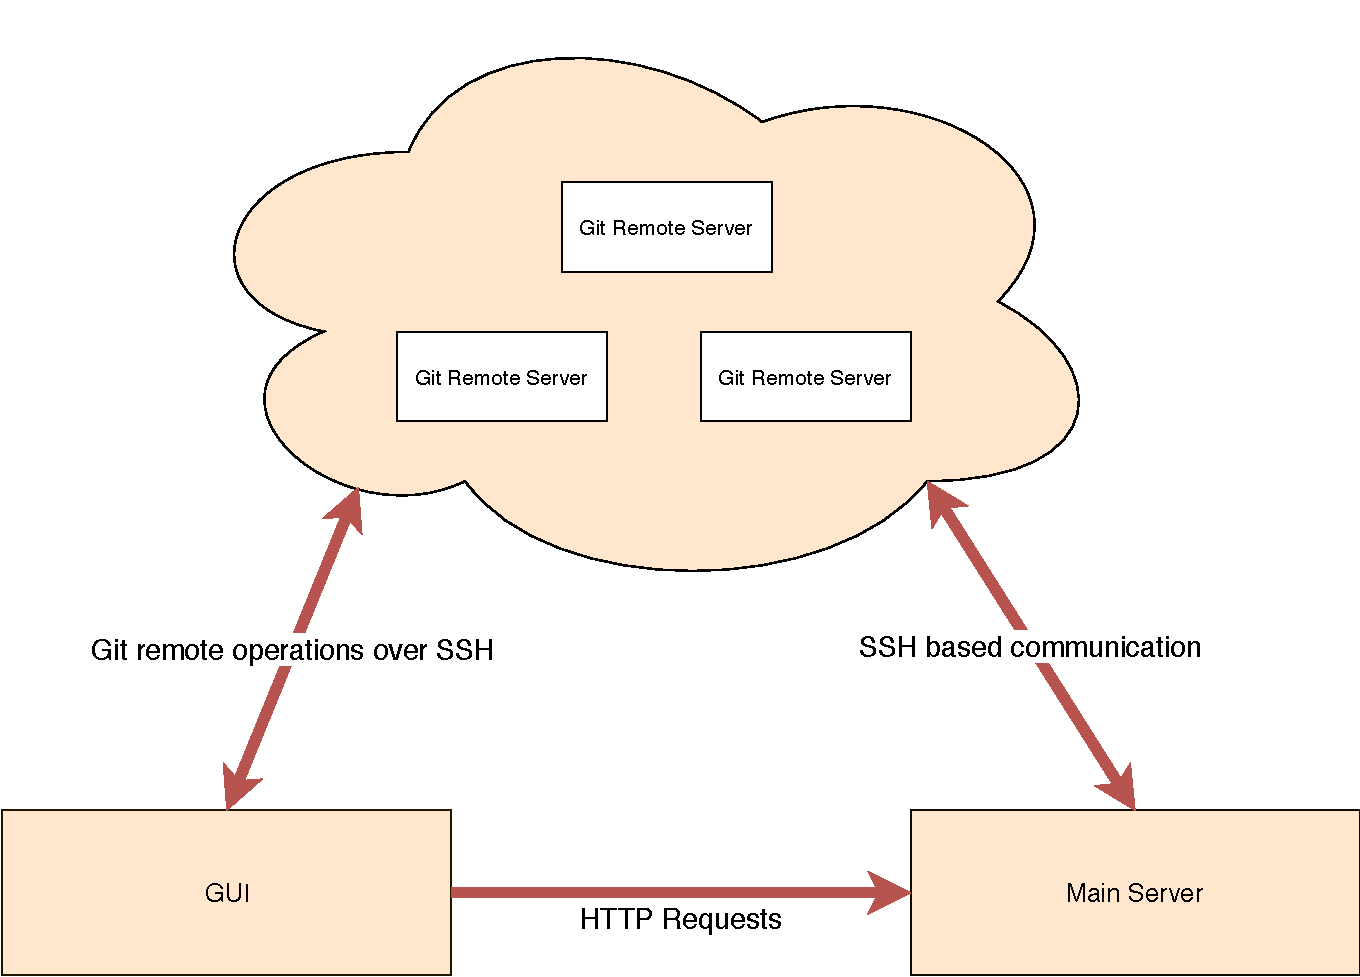
\includegraphics[scale = 0.5]{figures/highlevel.pdf}
    \caption{A high level representation of the architecture of the system. }
    \label{fig:highlevel}
\end{figure}

Figure \ref{fig:highlevel} shows an overview of the system. The three main components shown run on distinct machines communicating over the internet. The GUI is the graphical user interface that runs on the user's machine, and what they use to manipulate their repositories. 

The reader may recall that to take advantage of Git fully as a source control system the user must define a \emph{remote repository}. A repository hosted on a remote server which remains in sync with the local copy on the user's machine. The Git servers in Figure \ref{fig:highlevel} are the machines that host these remote repositories.

The final component is the main server. It does \emph{not} host remote repositories but manages the system as a whole. The main server keeps track of users and their repositories, as well as ensuring that the correct users have access to the correct repositories. 

\subsubsection{Git Servers and the Main server}

The user may ask whether this infrastructure is needed. There already exist many hosting services for Git repositories. GitHub, Gitlab and Bitbucket to name a few. However, the issue with using these remains to be our goal of automating as much as possible. To be able to set up SSH keys for the user we must have complete control over the backend infrastructure. 

Furthermore, this control allows for easy integration of new features in future. For example, we could introduce a new type of user such as a teacher who could have access to multiple repositories. To introduce such a role while relying on the stability of a third party service would be much more difficult.

Figure \ref{fig:highlevel} shows multiple Git servers; this demands some explanation. A reasonable question to ask is why is one not sufficient? The second of the two objectives for this project is to produce a scalable system. We must ask ourselves what happens if we start to get more users, creating more repositories. One server soon runs out of space. Moreover, our system is likely to slow when one Git server alone has multiple other machines communicating with it simultaneously.

For this reason, we spread the load of Git repositories over multiple machines. A future goal of this project is to have machines hosted in different regions around the world, and assign their repositories based on the location of users to make the system as efficient as possible.

Of course, having multiple servers hosting Git repositories presents its own set of challenges. For a user's machine to be able to communicate with a Git server, we must register its public SSH key on all the Git servers that host the user's repositories. One of the responsibilities of the main server is precisely this. To manage SSH keys, ensuring the right ones exist on the correct machines, which becomes more complicated when we realise that an SSH key is associated to a machine, not a user and that a user may work on multiple machines necessitating multiple keys.

The management of SSH keys is only one role assigned to the main server; it also creates Git repositories on the Git servers and manages users, keeps track of their repositories and handles all user authentication.

\subsubsection{GUI}

The GUI is the desktop application the end user interacts with and uses. Its primary responsibilities are to allow the user to manipulate the Git repository and visually display its current state.

\begin{figure} 
    \centering
    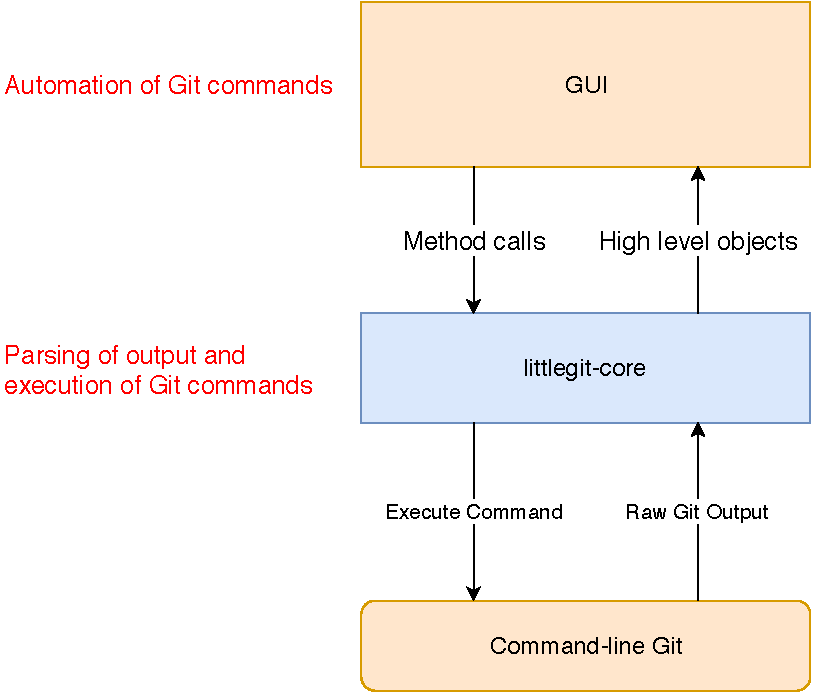
\includegraphics[scale = 0.5]{figures/gui-core.pdf}
    \caption{A representation of the interaction between the GUI and the littlegit-core }
    \label{fig:gui-layers}
\end{figure}
\subsubsection{ Low-level git library}

At this stage, it's prudent to mention the way both the GUI the main server interact with Git itself. This interaction happens through the medium of a library called the \textbf{littlegit-core} written for this system. It serves as a wrapper around the Git command line allowing interaction from a high-level language (discussed further in chapter 3) with the Git binary. The littlegit-core is responsible for executing git commands and parsing the output into useful high-level objects.

However, the reader should note that this layer performs none of the automation of Git which the system aims to achieve. This layer executes git commands then parses and returns the resulting output as Figure \ref{fig:gui-layers}.

Both the main server and GUI include the littlegit-core library as a dependency, allowing them to interact with Git repositories without interacting directly with the Git binary. 

We discuss the GUI's design and features in the following section.

\subsection{UI Design}
 
Early in the project, the interfaces of other Git GUIs were examined, exploring their strengths, weaknesses and most importantly, their common traits. The findings of this research are discussed here as well as a discussion of how the results impacted the design of this project's user interface.

The three main applications researched are the application SourceTree \cite{sourcetree} (mentioned earlier), GitKraken\cite{gitkraken} and GitK\cite{gitk}. Figures \ref{screenshot:sourcetree}, \ref{screenshot:gitkraken} and \ref{screenshot:gitk} show a screenshots of their main interfaces.

\fig{figures/sourcetree.png}{A screenshot of the main interface of the application SourceTree.}{screenshot:sourcetree}{0.3}

\fig{figures/gitkraken.png}{A screenshot of the main interface of the application GitKraken.}{screenshot:gitkraken}{0.3}

\fig{figures/gitk.png}{A screenshot of the main interface of the application GitK.}{screenshot:gitk}{0.3}

The first thing to note in looking at the interfaces is the clear common element being the Git graph. Though each has a different style and displays the information differently, the graphs are all large clear features of each interface. The decision was made to emulate the overall style in littlegit. The vertical graph, new commits on top with older commits in descending order below them. The reasoning here is that the Git history portrayed in this way conveys all needed information, but it is easy to present a simplified version (as was needed for littlegit) by simply omitting some of the information surrounding it.

Though other options were considered, Figure \ref{fig:horizontal-graph} shows an early design for an alternative graph. The idea was to emulate a timeline to help visualise the repository as being a series of snapshots of the code, allowing the user to navigate backwards and forwards along it. This idea however soon proved impractical, firstly visually representing branches in this model becomes messy and complicated, especially for more complex repositories. Furthermore, according to user testing \cite{horizontalScrolling}, users dislike horizontal scrolling.

\fig{figures/horizontal-graph.pdf}{An early design for the Git graph using horizontal scrolling.}{fig:horizontal-graph}{0.3}

Returning to our discussion of the other applications, the graphs of both SourceTree and GitK are relatively cramped. A large amount of information in very close proximity, this is especially true of GitK. On the other hand, GitKraken takes much more space to display the same information, a feature it was important for littlegit to emulate to ensure the data is clear and easy to understand.

The next point to make is that all three applications have lots of buttons and menus. By looking through all the buttons and options, it became clear that in a system that aims to automate as much as possible. The vast majority of the options were unneeded. For example, SourceTree has three separate buttons for pushing, pulling and fetching. The question littlegit asks is why? If there is something to push to the server, why not just do it on the users' behalf, and if there are no new changes on the server to be pulled, then why present the user with the option? This lead to the decision of having a popup dialogue appear when the user's local version is behind the server, giving them the option to update without the need to clutter the primary interface with the option.

Since this automation is taking place, it seems prudent to explicitly describe the Git workflow littlegit aims to present. The workflow is built around the commit, creating commits should drive everything else. Creating a commit causes changes to be pushed to the server, and the arrival of new commits on the server should cause the application to update the repository accordingly. Branches in this workflow are much less significant and are only used by littlegit internally when needed. With this in mind, looking back at SourceTree especially, it is very non-obvious how to create a new commit, something imperative to avoid in littlegit. 

Hence, creating new commits should be the primary operation the user sees when using the application. Furthermore, by looking at GitKraken and SourceTree in particular, the reader may also notice that many of the buttons on their left toolbars are merely the names of branches. In regular use clicking on them allows the user to check out these branches. Both applications also allow for using the graph to navigate between branches, allowing the user to click on the branch they wish to check out. With littlegit we aimed to expand this functionality, allowing the user to check out any commit in the history and handling this with branches internally without exposing this to the user.

\subsection {Designing for teenagers}\label{sec:teen-design}

There has been much research conducted on the topic of designing user interfaces for teenagers. Unfortunately, the orientation of much of that research was towards websites and mobile applications rather than desktop apps. A result of this is usually much discussion of the importance of social media integration and good mobile compatibility, neither of which apply to a desktop application such as littlegit.

However, many of the conclusions are useful, particularly a study by the Neilsen Norman Group concerning designing for teenagers \cite{teendesign}. 

One of the biggest influencers of this study on the design of littlegit is the conclusion that teenagers hate childish content, seeing it as patronising. For this reason, littlegit refrains from any unneeded graphics and multimedia. Where an explanation of functions are required, they are short and do not talk down to users.

Furthermore, the study suggests that the strategy mentioned earlier of reducing clutter on the main screen is the correct approach, including refraining from using flashy animations and graphics.

Lastly, a point continually emphasised by the study is that of fast loading speeds. Though this refers specifically to websites, the study highlights the impatience of teenagers while using the software.  The second objective of the project; therefore, of a scalable architecture which allows the application to work at speed is doubly important when considering the target audience.

\subsection{Final design before implementation}

The development of the software followed an iterative approach. This meant continually seeking feedback from others as the project continued. However, it was essential to have an initial design to aim for, taking into account the research above.

To do this the design software Sketch \cite{sketch,} was used to produce initial designs. These designs are included in Figures \ref{fig:design1} and \ref{design2}.

\fig{figures/design1.png}{The main screen of littlegit}{fig:design1}{0.11}

\fig{figures/design2.png}{The main screen of littlegit after a user clicks a commit from the graph.}{fig:design2}{0.11}



